%-*-latex-*-
\sectionthree{Linear Recursion}
\begin{python0}
from solutions import *; clear()
\end{python0}

Recall that a recursive function is a function that calls itself.
For instance here's Fibonacci again:
{\small
\begin{Verbatim}[frame=single,fontsize=\footnotesize]
def fib(n):
    if n == 0 or n == 1:
        return 1
    else:
        return fib(n - 1) + fib(n - 2)
\end{Verbatim}
}
Or in C/C++:
{\small
\begin{Verbatim}[frame=single,fontsize=\footnotesize]
int fib(int n)
{
    if (n == 0 || n == 1):
        return 1;
    else
        return fib(n - 1) + fib(n - 2);
}
\end{Verbatim}
}
Of course this is your standard first Fibonacci implementation. 
(Review your recursion notes from CISS245.)

The form of this function is derived from math.
In your math classes, one would write this function as
\[
f(n) = 
\begin{cases}
1                   & \text{if $n = 0, 1$} \\
f(n - 1) + f(n - 2) & \text{otherwise}
\end{cases}
\] 
In math, one would also say that this definition is piecewise ... 
because there are two pieces in the definition, right?

Each of the following cases
\[
f(0) = 1, \,\,\,\,\, f(1) = 1
\]
is usually called a \defone{base case}.
The case that has recursion
\[
f(n) = f(n - 1) + f(n - 2) , \,\,\,\,\, n > 1
\]
is called the \defone{recursive case} (duh).

How do you analyze the runtime of the above recursive function?
There are many types of recursion.
The above recursion
\[
f(n) = f(n - 1) + f(n - 2)
\]
is an example of a \defone{linear recursion} with fixed degree.
In the Fibonacci case, the \defone{degree} is 2 because
the parameters in the above are
\[
n, \,\,\,\,\, n - 1, \,\,\,\,\, n - 2
\]
and the largest difference between $n$ and the other parameters is $2$.
In general a degree 2 linear recurrrence $g(n)$ looks like this:
\[
g(n) = a \cdot g(n-1) + b \cdot g(n-2)
\]
where $a,b$ are constants.
A degree 3 linear recurrrence $h(n)$ looks like this:
\[
h(n) = a \cdot h(n-1) + b \cdot h(n-2) + c \cdot h(n-3)
\]
where $a,b,c$ are constants.



Here's what you do.
First you let 
\[
T(n)
\]
denote the total time to execute \verb!f(n)!
\textit{including} the time due to the recursive calls.
That includes the function call, the execution of the body (which can
include the time to execute the base case code or
the time due to the execution of the recursive calls)
and the return.

\begin{Verbatim}[frame=single,fontsize=\footnotesize]
def f(n):                                 t1
    if n == 0 or n == 1:                  t2
        return 1                          t3
    else:                                 t4 
        return f(n - 1) + f(n - 2)        t5
\end{Verbatim}

If the value of \verb!n! is \verb!0!, the above function returns 1.
Therefore
\begin{align*}
T(0) &= t_1 + t_2 + t_3 \\
T(1) &= t_1 + t_2 + t_3
\end{align*}
Since we're going to compute big-O, 
we're just going to write
\[
T(0) = T(1) = A
\]
for some constant $A$.
Now for the recursive case ...

What if $n > 1$?
Notice that your function call of \verb!f(n)! will have to make two calls:
a call to \verb!f(n - 1)! and then another call to \verb!f(n - 2)!.
Of course the time taken to execute \verb!f(n - 1)! is $T(n - 1)$.
And the time to execute 
\verb!f(n - 2)! is $T(n - 2)$.
When you get the results of \verb!f(n - 1)! and \verb!f(n - 2)!,
you have to add them together (which takes constant time)
and return the result (which also takes constant time).
Note the ... \textit{VERY IMPORTANT POINT} ... here:

Time $t_5$ depends on \verb!n! and therefore is \textit{not}
constant (with respect to \verb!n!).

Let me do this carefully (and slowly) and include everything.
You'll see later that most of the extra things/details to consider
are actually $O(1)$, i.e. constant time, and therefore 
not that crucial ... but you have to see it to see what's
happening. 
Here's the timing for $t_5$:
\begin{align*}
t_5 
&= \text{[time to compute $n - 1$]} + \text{[time to execute $f(n - 1)$]} \\
&\,\,\,\,\,  + \text{[time to compute $n - 2$]} + \text{[time to execute $f(n - 2)$]} \\
&\,\,\,\,\,  + \text{[time to add the return values of above]} \\
&\,\,\,\,\,  + \text{[time to return the sum]} \\
&= \text{[some constant]} + T(n-1) \\
&\,\,\,\,\,  + \text{[some constant]} + T(n-2) \\
&\,\,\,\,\,  + \text{[some constant]} \\
&\,\,\,\,\,  + \text{[some constant]} \\
&= T(n-1) + T(n-2) + B
\end{align*}
where $B$ is a constant.
(There are other details.
For instance time might be taken to store
the return value of the $f(n - 1)$ function call temporarily
before making the next function call of $f(n-2)$.
The time to store an integer value is constant and does not
change with $n$. 
So again this takes constant time.)

So for the case of $n > 1$,
\begin{align*}
T(n) 
&= t_1 + t_2 + t_4 + t_5 \\
&= t_1 + t_2 + t_4 + T(n-1) + T(n-2) + B \\
&= T(n-1) + T(n-2) + C
\end{align*}
for some constant $C$.

So, voil\`a, all together we have
\[
T(n) 
=
\begin{cases}
A                       & \text{ if $n = 0, 1$} \\
T(n - 1) + T(n - 2) + C & \text{ otherwise}
\end{cases}
\]

Hey! 
That does not give a formula for $T(n)$ in terms of $n$ ...
but in terms of $T(n - 1)$ and $T(n - 2)$!!!

The above \textit{recursive algorithm} gives a
\textit{recursive runtime formula}.

Or we say $T(n)$ satisfies a \defone{recurrence relation}.
Of course in analyzing runtimes, you prefer to put this
$T(n)$ into one of the standard runtime big-O classes such as
\[
O(1), \,\,\,\,\,
O(n^a), \,\,\,\,\,
O(n^b\ln^c n), \,\,\,\,\, 
O(c^n), ...
\]
so that you can tell how fast or slow it runs.
So I need to rewrite a recursive runtime formula into one that is not
recursive (yes, it's possible).
Such a formula is said to be a \defone{closed form formula}. 

\begin{comment}
Not to panic.
All you need to do is to understand
how to do numeric recursion (i.e. substitution).
For instance
\begin{align*}
T(5) 
&= T(4) + T(3) + d \\
&= (T(3) + T(2) + d) + (T(2) + T(1) + d) + d           & & \text{substitute} \\
&= T(3) + 2T(2) + T(1) + 3d                            & & \text{cleanup ...  ur mom told u right?} \\
&= (T(2) + T(1) + d) + 2(T(1) + T(0) + d) + T(1) + 3d  & & \text{substitute} \\
&= T(2) + 4T(1) + 2T(0) + 6d                           & & \text{cleanup} \\
&= T(1) + T(0) + d + 4T(1) + 2T(0) + 6d                & & \text{substitute} \\
&= 5T(1) + 3T(0) + 7d                                  & & \text{cleanup}
\end{align*}

This is all well and good ... but we need $T(n)$, not $T(5)$!!!
Ultimately do you see that $T(n)$ must be of the form:
\[
T(n) = \text{BLAH1} \cdot T(1) + \text{BLAH2} \cdot T(0) + \text{BLAH3} \cdot d
\]
where BLAH1, BLAH2 and BLAH3 must be formulas involving $n$.
Ultimately we're going to ditch the constants $T(1)$, $T(0)$ and $d$.
What matters is really BLAH1, BLAH2, BLAH3.
It turns out that BLAH1 and BLAH2 are of the form
\[
\text{(some constant)}^n
\]
One of the constants is approximately 1.618 while the other is
approximately -0.618.

That already tells you that the runtime of the above 
algorithm to compute the $n$--th Fibonacci number is pretty bad:
it's ...
\[
\text{exponential!!!}
\]

That's why if you use the above to compute $f(i)$ for $i = 0, 1, 2, ...$,
you will see that your program will slow down to almost a grinding halt
after $i=50$.

It turns out that for such problems you can rewrite the program to run in 
linear time, i.e., $O(n)$.
In fact that there are \textit{several} different ways to do that.
I'll talk about this is another set of notes 
(on techniques for re-designing algorithms to
improving runtime) since for this set of notes
I'm only going to focus on measuring runtimes.

Of course I still have not explained how I got this mysterious 1.618.
But I'm going to take a pause here and give you some exercises first ...

First of all, it's clear that a \textit{recursive algorithm} like the above
will give you a corresponding \textit{recursing runtime}.
Here are some exercises to verify that. 


\newpage
\begin{ex}
Using the same technique above, compute a recursive runtime
for the following algorithm.
(Don't worry about writing the formula in closed form.)
\begin{Verbatim}[frame=single,fontsize=\footnotesize]
def f(n):
    if n == 0: 
        return 1
    elif n == 1:
        return 3
    else:
         return 2 * f(n - 1) + 3 * f(n - 2)
\end{Verbatim}
\end{ex}

\newpage
\begin{ex}
Using the same technique above, compute a recursive runtime
for the following algorithm.
(Don't worry about writing the formula in closed form.)
\begin{Verbatim}[frame=single,fontsize=\footnotesize]
def f(n):
    if n == 0: 
        return 5
    else:
        return 7 * f(n - 1) + 2 
\end{Verbatim}
\end{ex}


\newpage
\begin{ex}
Using the same technique above, compute a recursive runtime
for the following algorithm.
(Don't worry about writing the formula in closed form.)
\begin{Verbatim}[frame=single,fontsize=\footnotesize]
def f(n):
    if n == 0: 
        return 7
    elif n == 1:
        return 10
    else:
        return n * f(n - 1) +  f(n - 2)
\end{Verbatim}
\end{ex}



\newpage
\begin{ex}
Using the same technique above, compute a recursive runtime
for the following algorithm.
(Don't worry about writing the formula in closed form.)
\begin{Verbatim}[frame=single,fontsize=\footnotesize]
def f(n):
    if n == 0: 
        return 7
    elif n == 1:
        return 10
    else:
        return f(n - 1) * f(n - 2)
\end{Verbatim}
\end{ex}

%[MORE EXERCISES]

\end{comment}

%\newpage
%\subsection*{Solutions}
%
\newpage
\section*{Solutions}
Solution to Exercise \ref{ex:dfa0}\labeltext{}{sol:dfa0}.

\tinysidebar{\debug{exercises/{dfa0/answer.tex}}}

    Solution not provided.
    

\newpage

Solution to Exercise \ref{ex:dfa1}\labeltext{}{sol:dfa1}.

\tinysidebar{\debug{exercises/{dfa1/answer.tex}}}
  The ID computation is
  \begin{align*}
    (q_0, aba)
    &\vdash (\delta(q_0, a), ba) = (q_0, ba) \\ 
    &\vdash (\delta(q_0, b), a) = (q_1, a) \\
    &\vdash (\delta(q_1, a), \ep) = (q_0, \ep)
  \end{align*}
  $q_0$ is not an accept state. Therefore $aba$ is not accepted.


\newpage

Solution to Exercise \ref{ex:dfa4}\labeltext{}{sol:dfa4}.

\tinysidebar{\debug{exercises/{dfa4/answer.tex}}}

    Solution not provided.
    

\newpage

Solution to Exercise \ref{ex:dfa5}\labeltext{}{sol:dfa5}.

\tinysidebar{\debug{exercises/{dfa5/answer.tex}}}

    Solution not provided.
    

\newpage

Solution to Exercise \ref{ex:implementing-a-single-dfa0}\labeltext{}{sol:implementing-a-single-dfa0}.

\tinysidebar{\debug{exercises/{implementing-a-single-dfa0/answer.tex}}}

    Solution not provided.
    

\newpage

Solution to Exercise \ref{ex:nfastatediag0}\labeltext{}{sol:nfastatediag0}.

\tinysidebar{\debug{exercises/{nfastatediag0/answer.tex}}}

    Solution not provided.
    

\newpage

Solution to Exercise \ref{ex:nfastatediag1}\labeltext{}{sol:nfastatediag1}.

\tinysidebar{\debug{exercises/{nfastatediag1/answer.tex}}}

    Solution not provided.
    

\newpage

Solution to Exercise \ref{ex:nfastatediag2}\labeltext{}{sol:nfastatediag2}.

\tinysidebar{\debug{exercises/{nfastatediag2/answer.tex}}}

    Solution not provided.
    

\newpage

Solution to Exercise \ref{ex:nfastatediag3}\labeltext{}{sol:nfastatediag3}.

\tinysidebar{\debug{exercises/{nfastatediag3/answer.tex}}}

    Solution not provided.
    

\newpage

Solution to Exercise \ref{ex:nfastatediag4}\labeltext{}{sol:nfastatediag4}.

\tinysidebar{\debug{exercises/{nfastatediag4/answer.tex}}}

    Solution not provided.
    

\newpage

Solution to Exercise \ref{ex:nfastatediag5}\labeltext{}{sol:nfastatediag5}.

\tinysidebar{\debug{exercises/{nfastatediag5/answer.tex}}}

    Solution not provided.
    

\newpage

Solution to Exercise \ref{ex:nfastatediag6}\labeltext{}{sol:nfastatediag6}.

\tinysidebar{\debug{exercises/{nfastatediag6/answer.tex}}}

    Solution not provided.
    

\newpage

Solution to Exercise \ref{ex:nfastatediag7}\labeltext{}{sol:nfastatediag7}.

\tinysidebar{\debug{exercises/{nfastatediag7/answer.tex}}}

    Solution not provided.
    

\newpage

Solution to Exercise \ref{ex:nfastatediag8}\labeltext{}{sol:nfastatediag8}.

\tinysidebar{\debug{exercises/{nfastatediag8/answer.tex}}}

    Solution not provided.
    

\newpage

Solution to Exercise \ref{ex:nfastatediag9}\labeltext{}{sol:nfastatediag9}.

\tinysidebar{\debug{exercises/{nfastatediag9/answer.tex}}}

    Solution not provided.
    

\newpage

Solution to Exercise \ref{ex:nfastatediag10}\labeltext{}{sol:nfastatediag10}.

\tinysidebar{\debug{exercises/{nfastatediag10/answer.tex}}}

    Solution not provided.
    

\newpage

Solution to Exercise \ref{ex:nfastatediag11}\labeltext{}{sol:nfastatediag11}.

\tinysidebar{\debug{exercises/{nfastatediag11/answer.tex}}}

    Solution not provided.
    

\newpage

Solution to Exercise \ref{ex:nfastatediag12}\labeltext{}{sol:nfastatediag12}.

\tinysidebar{\debug{exercises/{nfastatediag12/answer.tex}}}

    Solution not provided.
    

\newpage

Solution to Exercise \ref{ex:nfastatediag13}\labeltext{}{sol:nfastatediag13}.

\tinysidebar{\debug{exercises/{nfastatediag13/answer.tex}}}

    Solution not provided.
    

\newpage

Solution to Exercise \ref{ex:nfa0}\labeltext{}{sol:nfa0}.

\tinysidebar{\debug{exercises/{nfa0/answer.tex}}}
The formal definition of this NFA is $(\Sigma, Q, q_0, \delta, F)$ where
\begin{tightlist}
\li $\Sigma = \{a,b\}$
\li $Q = \{q_0\}$
\li $\delta$ is the function
\[
\delta : Q \times \Sigma_\epsilon \rightarrow P(Q)
\]
given by
\begin{align*}
  \delta(q_0, \epsilon) &= \{\} \\
  \delta(q_0, a) &= \{\} \\
  \delta(q_0, b) &= \{\} 
\end{align*}
\end{tightlist}


\newpage

Solution to Exercise \ref{ex:nfa1}\labeltext{}{sol:nfa1}.

\tinysidebar{\debug{exercises/{nfa1/answer.tex}}}

    Solution not provided.
    

\newpage

Solution to Exercise \ref{ex:nfa2}\labeltext{}{sol:nfa2}.

\tinysidebar{\debug{exercises/{nfa2/answer.tex}}}

    Solution not provided.
    

\newpage

Solution to Exercise \ref{ex:nfa3}\labeltext{}{sol:nfa3}.

\tinysidebar{\debug{exercises/{nfa3/answer.tex}}}

    Solution not provided.
    

\newpage

Solution to Exercise \ref{ex:nfa4}\labeltext{}{sol:nfa4}.

\tinysidebar{\debug{exercises/{nfa4/answer.tex}}}

    Solution not provided.
    

\newpage

Solution to Exercise \ref{ex:nfa5}\labeltext{}{sol:nfa5}.

\tinysidebar{\debug{exercises/{nfa5/answer.tex}}}

    Solution not provided.
    

\newpage

Solution to Exercise \ref{ex:dfa-as-powerful-as-nfa0}\labeltext{}{sol:dfa-as-powerful-as-nfa0}.

\tinysidebar{\debug{exercises/{dfa-as-powerful-as-nfa0/answer.tex}}}
Here's the solution.
Let $\delta$ denote the transition function of $N$.
Note that 
\begin{align*}
  \delta(q_0, \epsilon) = \{\} \\
  \delta(q_0, a) = \{\} \\
  \delta(q_0, b) = \{\} 
\end{align*}
First of all the states are labeled as all the subsets of $\{q_0\}$.


\begin{center}
\begin{tikzpicture}[>=triangle 60,shorten >=0.5pt,node distance=2cm,auto,initial text=, double distance=2pt]
\node[state] (A) at (  0,  0) {$\{q_0\}$};
\node[state] (B) at (  3,  0) {$\{\}$};

\path[->]

;
\end{tikzpicture}
\end{center}
    


The start state is the $\epsilon$-closure of $\{q_0\}$.
However in $N$, there are no $\epsilon$--transitions out of 
$q_0$.
So the $\epsilon$-closure of $\{q_0\}$ is in fact $\{q_0\}$, i.e.
$\overline{\{q_0\}} = \{q_0\}$
The $\DFA$ is now this:


\begin{longtable}{|r||r|r|r|r|r|}
\hline 
         & $w_1$ & $w_2$ & $w_3$ & $w_4$ & $\ldots$ \\ \hline \hline 
$M_1$    &       &       &       &       &          \\ \hline 
$M_2$    &       &       &       &       &          \\ \hline 
$M_3$    &       &       &       &       &          \\ \hline 
$M_4$    &       &       &       &       &          \\ \hline 
$\ldots$ &       &       &       &       &          \\ \hline 
\end{longtable}
        


Now I will compute the $a$--transition of the state $\{q_0\}$.
Let $\delta^\DFA$ denote the transition function of the $\DFA$
that we're building.
Then
\begin{align*}
\delta( \{q_0, a\} ) 
&= \overline{ \bigcup_{q \in \{q_0\}} \delta(q, a)} \\
&= \overline{ \delta(q_0, a) } \\
&= \overline{ \emptyset } \\
&= \emptyset
\end{align*}
The (incomplete) $\DFA$ now looks like this:


\begin{longtable}{|r||r|r|r|r|r|}
\hline 
         & $w_1$ & $w_2$ & $w_3$ & $w_4$ & $\ldots$ \\ \hline \hline 
$M_1$    & 0     & 0     & 1     & 0     & ...      \\ \hline 
$M_2$    & 1     & 0     & 1     & 1     & ...      \\ \hline 
$M_3$    & 0     & 1     & 1     & 1     & ...      \\ \hline 
$M_4$    & 1     & 0     & 1     & 1     & ...      \\ \hline 
$\ldots$ &       &       &       &       &          \\ \hline 
\end{longtable}
        


Using the same reasoning we have

\begin{center}
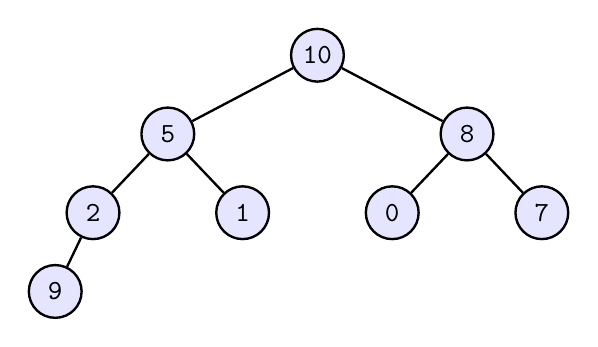
\begin{tikzpicture}

\fill[blue!10] (0.0, 0.0) circle (0.35);
\node [line width=0.03cm,black,minimum size=0.6699999999999999cm,draw,circle] at (0.0,0.0)(10){};\draw (0.0, 0.0) node[color=black] {\texttt{10}};
\fill[blue!10] (-1.9, -1.0) circle (0.35);
\node [line width=0.03cm,black,minimum size=0.6699999999999999cm,draw,circle] at (-1.9,-1.0)(5){};\draw (-1.9, -1.0) node[color=black] {\texttt{5}};
\fill[blue!10] (1.9, -1.0) circle (0.35);
\node [line width=0.03cm,black,minimum size=0.6699999999999999cm,draw,circle] at (1.9,-1.0)(8){};\draw (1.9, -1.0) node[color=black] {\texttt{8}};
\fill[blue!10] (-2.85, -2.0) circle (0.35);
\node [line width=0.03cm,black,minimum size=0.6699999999999999cm,draw,circle] at (-2.85,-2.0)(2){};\draw (-2.85, -2.0) node[color=black] {\texttt{2}};
\fill[blue!10] (-0.95, -2.0) circle (0.35);
\node [line width=0.03cm,black,minimum size=0.6699999999999999cm,draw,circle] at (-0.95,-2.0)(1){};\draw (-0.95, -2.0) node[color=black] {\texttt{1}};
\fill[blue!10] (0.95, -2.0) circle (0.35);
\node [line width=0.03cm,black,minimum size=0.6699999999999999cm,draw,circle] at (0.95,-2.0)(0){};\draw (0.95, -2.0) node[color=black] {\texttt{0}};
\fill[blue!10] (2.85, -2.0) circle (0.35);
\node [line width=0.03cm,black,minimum size=0.6699999999999999cm,draw,circle] at (2.85,-2.0)(7){};\draw (2.85, -2.0) node[color=black] {\texttt{7}};
\fill[blue!10] (-3.33, -3.0) circle (0.35);
\node [line width=0.03cm,black,minimum size=0.6699999999999999cm,draw,circle] at (-3.33,-3.0)(9){};\draw (-3.33, -3.0) node[color=black] {\texttt{9}};\draw[line width=0.03cm,black] (10) to  (5);
\draw[line width=0.03cm,black] (10) to  (8);
\draw[line width=0.03cm,black] (5) to  (2);
\draw[line width=0.03cm,black] (5) to  (1);
\draw[line width=0.03cm,black] (8) to  (0);
\draw[line width=0.03cm,black] (8) to  (7);
\draw[line width=0.03cm,black] (2) to  (9);
\end{tikzpicture}

\end{center}



It's easy to see that in the DFA, the $a$--
and $b$--transitions from the state $\{\}$ goes back to itself.
Therefore the completed DFA is this:


\begin{center}
\begin{tikzpicture}[>=triangle 60,shorten >=0.5pt,node distance=2cm,auto,initial text=, double distance=2pt]
\node[state,initial] (A) at (  0,  0) {$\{q_0\}$};
\node[state] (B) at (  3,  0) {$\{\}$};

\path[->]
(A) edge [bend left=0,pos=0.5,above] node {$a,b$} (B)
(B) edge [loop above] node {$a,b$} ()

;
\end{tikzpicture}
\end{center}
    



\newpage

Solution to Exercise \ref{ex:dfa-as-powerful-as-nfa1}\labeltext{}{sol:dfa-as-powerful-as-nfa1}.

\tinysidebar{\debug{exercises/{dfa-as-powerful-as-nfa1/answer.tex}}}

    Solution not provided.
    

\newpage

Solution to Exercise \ref{ex:dfa-as-powerful-as-nfa2}\labeltext{}{sol:dfa-as-powerful-as-nfa2}.

\tinysidebar{\debug{exercises/{dfa-as-powerful-as-nfa2/answer.tex}}}

    Solution not provided.
    

\newpage

Solution to Exercise \ref{ex:dfa-as-powerful-as-nfa3}\labeltext{}{sol:dfa-as-powerful-as-nfa3}.

\tinysidebar{\debug{exercises/{dfa-as-powerful-as-nfa3/answer.tex}}}

    Solution not provided.
    

\newpage

Solution to Exercise \ref{ex:dfa-as-powerful-as-nfa4}\labeltext{}{sol:dfa-as-powerful-as-nfa4}.

\tinysidebar{\debug{exercises/{dfa-as-powerful-as-nfa4/answer.tex}}}

    Solution not provided.
    

\newpage

Solution to Exercise \ref{ex:closure0}\labeltext{}{sol:closure0}.

\tinysidebar{\debug{exercises/{closure0/answer.tex}}}

    Solution not provided.
    

\newpage

Solution to Exercise \ref{ex:closure1}\labeltext{}{sol:closure1}.

\tinysidebar{\debug{exercises/{closure1/answer.tex}}}

    Solution not provided.
    

\newpage

Solution to Exercise \ref{ex:closure2}\labeltext{}{sol:closure2}.

\tinysidebar{\debug{exercises/{closure2/answer.tex}}}

    Solution not provided.
    

\newpage

Solution to Exercise \ref{ex:closure3}\labeltext{}{sol:closure3}.

\tinysidebar{\debug{exercises/{closure3/answer.tex}}}

    Solution not provided.
    

\newpage

Solution to Exercise \ref{ex:closure4}\labeltext{}{sol:closure4}.

\tinysidebar{\debug{exercises/{closure4/answer.tex}}}

    Solution not provided.
    

\newpage

Solution to Exercise \ref{ex:closure5}\labeltext{}{sol:closure5}.

\tinysidebar{\debug{exercises/{closure5/answer.tex}}}

    Solution not provided.
    

\newpage

Solution to Exercise \ref{ex:closure6}\labeltext{}{sol:closure6}.

\tinysidebar{\debug{exercises/{closure6/answer.tex}}}

    Solution not provided.
    

\newpage

Solution to Exercise \ref{ex:closure7}\labeltext{}{sol:closure7}.

\tinysidebar{\debug{exercises/{closure7/answer.tex}}}

    Solution not provided.
    

\newpage

Solution to Exercise \ref{ex:closure8}\labeltext{}{sol:closure8}.

\tinysidebar{\debug{exercises/{closure8/answer.tex}}}

    Solution not provided.
    

\newpage

Solution to Exercise \ref{ex:closure9}\labeltext{}{sol:closure9}.

\tinysidebar{\debug{exercises/{closure9/answer.tex}}}

    Solution not provided.
    

\newpage

Solution to Exercise \ref{ex:closure10}\labeltext{}{sol:closure10}.

\tinysidebar{\debug{exercises/{closure10/answer.tex}}}

    Solution not provided.
    

\newpage

Solution to Exercise \ref{ex:closure11}\labeltext{}{sol:closure11}.

\tinysidebar{\debug{exercises/{closure11/answer.tex}}}

    Solution not provided.
    

\newpage

Solution to Exercise \ref{ex:closure12}\labeltext{}{sol:closure12}.

\tinysidebar{\debug{exercises/{closure12/answer.tex}}}

    Solution not provided.
    

